\documentclass[11pt,a4paper]{article}
\input{../../shared/preamble}
\SpeedHeader{Geometry}{2}

\begin{document}

\SpeedTitleBlock{Daily Geometry Drill \#2 --- Answers \& Investigations}{Henry Koduthore}
\noindent\textit{New toolkit today: Circle Equations $\cdot$ Tangents $\cdot$ Line--Circle Tests $\cdot$ Chord Lengths.}

%═══════════════════════════════════════════════════════════════════════════════
\section*{Section A \quad Rapid Recognition}
%═══════════════════════════════════════════════════════════════════════════════
\begin{enumerate}

%── A1 ──────────────────────────────────────────────────────────────────────────
\item Write down the centre of the circle $\;x^2 + y^2 - 6x - 8y + 24 = 0$.

\ans{"$(3,4)$"}
\method{Complete the square: $(x-3)^2+(y-4)^2=25-24=1$, so centre $(3,4)$, radius $1$.}
\inv{In $x^2+y^2+2gx+2fy+c=0$ the centre is $(-g,-f)$ and here $2g=-6$, $2f=-8$, so $g=-3$, $f=-4$ --- centre $(3,4)$ \checkmark. \textbf{If the coefficients of $x^2,y^2$ are not $1$, divide through first so they are, then read the centre.}}

%── A2 ───────────────────────────────────────────────────────────────────────
\item For which value of $k$ does $\;x^2+y^2-6x+4y+k=0$ represent a circle of radius $5$?

\ans{$-12$}
\method{Complete the square: $(x-3)^2+(y+2)^2=13-k$. Radius $5$ needs $13-k=25$, so $k=-12$.}
\inv{For which $k$ is this a real circle at all, and what does the equation describe at the boundary value?}

%── A3 ──────────────────────────────────────────────────────────────────────────
\item Write down the equation of the circle with centre $(2,-1)$ and radius $5$.

\ans{"$x^2+y^2-4x+2y-20=0$"}
\method{$(x-2)^2+(y+1)^2=25$ expands to $x^2+y^2-4x+2y+5=25$, i.e. $x^2+y^2-4x+2y-20=0$.}
\inv{Reading back: $2g=-4\Rightarrow g=-2$ (centre $x=2$), $2f=2\Rightarrow f=1$ (centre $y=-1$), $r=\sqrt{g^2+f^2-c}=\sqrt{4+1+20}=5$ \checkmark. \textbf{Rewrite for centre $(2,-1)$ radius $2$: what becomes of the constant?} $\;x^2+y^2-4x+2y+1=0$.}

%── A4 ──────────────────────────────────────────────────────────────────────────
\item Write down the radius of the circle $\;x^2 + y^2 - 4x + 6y - 12 = 0$.

\ans{$5$}
\method{Complete the square: $(x-2)^2+(y+3)^2=4+9+12=25$, so $r=5$.}
\inv{Formula: $g=-2,f=3$, $r=\sqrt{4+9+12}=5$ \checkmark. \textbf{All these squares are perfect: $5^2,4^2,3^2$. What radius would an {\em irrational} answer look like, and would that stop a clean distance test?} Only the appearance changes; the distance test still works.}

%── A5 ──────────────────────────────────────────────────────────────────────────
\item The point $(x,4)$ lies on the circle $\;x^2 + y^2 = 25$ with $x > 0$. Find $x$.

\ans{$3$}
\method{$x^2+4^2=25\Rightarrow x^2=9\Rightarrow x=\pm3$; take $+3$.}
\inv{Both $(3,4)$ and $(-3,4)$ lie on the circle --- the $x>0$ condition kills one branch. \textbf{List all lattice points $(x,y)$ on $x^2+y^2=25$.} $(0,\pm5),(\pm3,\pm4),(\pm4,\pm3),(\pm5,0)$.}

%── A6 ──────────────────────────────────────────────────────────────────────────
\item The radius from the origin to the point $(3,4)$ on $\;x^2+y^2=25$ has what gradient?

\ans{$\frac{4}{3}$}
\method{Gradient $=\frac{4-0}{3-0}=\frac43$.}
\inv{The radius is the line joining centre to the point. \textbf{Gradient of the perpendicular radius to $(3,-4)$?} $-\frac43$.}

%── A7 ──────────────────────────────────────────────────────────────────────────
\item The tangent to $\;x^2 + y^2 = 25$ at the point $(3,4)$ has what gradient?

\ans{$-\frac{3}{4}$}
\method{Tangent $\perp$ radius, and radius gradient is $\frac43$, so tangent gradient $=-\frac{1}{4/3}=-\frac34$.}
\inv{The tangent line is $3x+4y=25$ (via $xx_1+yy_1=r^2$). \textbf{Does it pass through $(3,4)$?} $9+16=25$ \checkmark. \textbf{What is its $x$-intercept?} $x=25/3$.}

%── A8 ───────────────────────────────────────────────────────────────────────
\item Write down the equation of the circle with centre $(3,-4)$ that passes through the origin.

\ans{$(x-3)^2+(y+4)^2=25$}
\method{The radius is the distance from $(3,-4)$ to $(0,0)$, which is $5$.}
\inv{Expanded, the equation has no constant term. Explain why every circle through the origin has $c=0$ in the form $x^2+y^2+2gx+2fy+c=0$.}

%── A9 ──────────────────────────────────────────────────────────────────────────
\item The centre of $\;x^2+y^2-6x-8y+24=0$ is $(3,4)$. Find the perpendicular distance of this centre from the line $\;4x + 3y - 9 = 0$.

\ans{$3$}
\method{Distance $=\frac{|4(3)+3(4)-9|}{\sqrt{4^2+3^2}}=\frac{|12+12-9|}{5}=\frac{15}{5}=3$.}
\inv{This is Day 1's perpendicular-distance formula applied to a centre. Since $d=3>r=1$, the line misses the circle: find the line parallel to $4x+3y-9=0$ that is tangent to the circle on the near side.}

%── A10 ─────────────────────────────────────────────────────────────────────────
\item A chord of the circle $\;x^2+y^2=25$ is at perpendicular distance $3$ from the origin. Find the length of the chord.

\ans{$8$}
\method{Half-chord $=\sqrt{r^2-d^2}=\sqrt{25-9}=\sqrt{16}=4$; full length $=8$.}
\inv{The perpendicular from the centre to a chord bisects it --- the half-chord formula. \textbf{If the distance were $4$, the length is $6$; if $5$,\  it degenerates to a tangent. Check both.} The chord shrinks to a point exactly when $d=r$.}

\end{enumerate}

%═══════════════════════════════════════════════════════════════════════════════
\section*{Section B \quad Manipulation Drills}
%═══════════════════════════════════════════════════════════════════════════════
\begin{enumerate}

%── B1 ──────────────────────────────────────────────────────────────────────────
\item Which of the following is the equation of the circle with centre $(3,-2)$ and radius $4$?
\begin{itemize}
\item[A)] $x^2+y^2-6x+4y-3=0$
\item[B)] $x^2+y^2-6x+4y+9=0$
\item[C)] $x^2+y^2+6x-4y-3=0$
\item[D)] $x^2+y^2-6x-4y-3=0$
\end{itemize}

\ans{A) $x^2+y^2-6x+4y-3=0$}
\method{$(x-3)^2+(y+2)^2=16$ gives $x^2+y^2-6x+4y+13=16$, i.e. $x^2+y^2-6x+4y-3=0$.}
\inv{Only A has both the $x$-coefficient $-6$ (centre $x=3$) and the $y$-coefficient $+4$ (centre $y=-2$). \textbf{B has the right coefficients but the wrong constant $+9$; what radius would that give?} $r=\sqrt{9+4-9}=2$.}

%── B2 ──────────────────────────────────────────────────────────────────────────
\item The circle $\;x^2+y^2+2x-4y-11=0$ has what radius?
\begin{itemize}
\item[A)] $2$
\item[B)] $3$
\item[C)] $4$
\item[D)] $\sqrt{5}$
\end{itemize}

\ans{C) $4$}
\method{$(x+1)^2+(y-2)^2=1+4+11=16$, so $r=4$.}
\inv{Complete the square exactly: $x^2+2x=(x+1)^2-1$ and $y^2-4y=(y-2)^2-4$, so $(x+1)^2+(y-2)^2=11+1+4=16$ and $r=4$ \checkmark. With $g=1,f=-2,c=-11$ the formula reads $r=\sqrt{g^2+f^2-c}=\sqrt{1+4+11}$. \textbf{Option D ($\sqrt{5}$) traps students who drop the constant $11$ (leaving $r^2=1+4=5$) or flip the sign of $c$; keep the sign fixed through the whole square.}}

%── B3 ──────────────────────────────────────────────────────────────────────────
\item The point $(1,2)$ lies on the circle $\;x^2+y^2=5$. The equation of the tangent to the circle at $(1,2)$ is?
\begin{itemize}
\item[A)] $y = -\frac{1}{2}x + \frac{5}{2}$
\item[B)] $y = 2x$
\item[C)] $y = -2x + 5$
\item[D)] $y = \frac{1}{2}x$
\end{itemize}

\ans{A) $y = -\frac12 x + \frac52$}
\method{Radius gradient $=\frac21=2$; tangent gradient $=-\frac12$; through $(1,2)$: $y-2=-\frac12(x-1)\Rightarrow y=-\frac12x+\frac52$.}
\inv{Option B is the radius line itself, option C negates the radius gradient without inverting it, and option D inverts without negating. The split-variable form $xx_1+yy_1=r^2$ gives $x+2y=5$ directly.}

%── B4 ──────────────────────────────────────────────────────────────────────────
\item A circle of form $\;x^2+y^2+2gx+2fy+c=0$ passes through the origin. Deduce $c$.
\begin{itemize}
\item[A)] $c = 1$
\item[B)] $c = 0$
\item[C)] $c = g + f$
\item[D)] $c = -1$
\end{itemize}

\ans{B) $c=0$}
\method{At the origin $(0,0)\in$ circle means $0+0+0+0+c=0$ --- the constant term is the value of the LHS at the origin, so $c=0$.}
\inv{\textbf{Circle $x^2+y^2=25$ has $c=-25$ and indeed does {\em not} pass through the origin.} The constant records the origin's membership: $c=0\Leftrightarrow$ origin on the circle.}

%── B5 ──────────────────────────────────────────────────────────────────────────
\item The perpendicular distance from the centre of $\;x^2+y^2=25$ to the line $\;y = 2x + 3$ is?
\begin{itemize}
\item[A)] $\dfrac{3}{\sqrt{5}}$
\item[B)] $\dfrac{3}{5}$
\item[C)] $3$
\item[D)] $2$
\end{itemize}

\ans{A) $\frac{3}{\sqrt5}$}
\method{Line $2x-y+3=0$; distance from $(0,0)$ $=\frac{|3|}{\sqrt{2^2+(-1)^2}}=\frac{3}{\sqrt5}$.}
\inv{\textbf{Compare with $r=5$: $\frac{3}{\sqrt5}<5$, so the line cuts the circle.} This is exactly the Day-1 formula put to the new line--circle test.}

%── B6 ──────────────────────────────────────────────────────────────────────────
\item Which of the following is a tangent to the circle $\;x^2+y^2=4$?
\begin{itemize}
\item[A)] $y = x + 2\sqrt{2}$
\item[B)] $y = x + 4$
\item[C)] $y = 2x + 2$
\item[D)] $y = 2x + 4$
\end{itemize}

\ans{A) $y = x + 2\sqrt2$}
\method{Line $x-y+2\sqrt2=0$ has distance from origin $\frac{2\sqrt2}{\sqrt2}=2=r$ --- tangent. The others give $\frac{4}{\sqrt2}=2\sqrt2$, $\frac2{\sqrt5}$, $\frac4{\sqrt5}$, none equal to $2$.}
\inv{Only option A places the origin exactly $r$ away. \textbf{Check B: $y=x+4$ has distance $2\sqrt2>2$, so it misses the circle.} Shifting a tangent line a little breaks tangency --- distance must {\em equal} $r$.}

%── B7 ──────────────────────────────────────────────────────────────────────────
\item A chord of the circle $\;x^2+y^2=13$ has length $4\sqrt{3}$. What is the perpendicular distance of the chord from the centre?
\begin{itemize}
\item[A)] $3$
\item[B)] $2$
\item[C)] $\sqrt{5}$
\item[D)] $1$
\end{itemize}

\ans{D) $1$}
\method{Half-chord $=2\sqrt3$; $(2\sqrt3)^2=13-d^2\Rightarrow 12=13-d^2\Rightarrow d^2=1\Rightarrow d=1$.}
\inv{\textbf{Fallback: remember $(\text{half-chord})^2+(\perp\,\text{dist})^2=r^2$.} Statement C ($\sqrt5$) is the trap of $13-8$ instead of $13-12$.}

%── B8 ──────────────────────────────────────────────────────────────────────────
\item The line $\;y = mx + 4$ is a tangent to the circle $\;x^2+y^2=4$. Find the two possible values of $m$.
\begin{itemize}
\item[A)] $\pm 1$
\item[B)] $\pm \sqrt{3}$
\item[C)] $\pm 2$
\item[D)] $\pm \sqrt{2}$
\end{itemize}

\ans{B) $\pm \sqrt3$}
\method{Line $mx-y+4=0$; tangency requires $\frac{|4|}{\sqrt{m^2+1}}=2\Rightarrow\sqrt{m^2+1}=2\Rightarrow m^2=3\Rightarrow m=\pm\sqrt3$.}
\inv{Both tangent lines pass through $(0,4)$, symmetric about the $y$-axis --- the two tangents from an external point. \textbf{How long is each tangent segment from $(0,4)$ to its touch point?} $\sqrt{16-4}=\sqrt{12}=2\sqrt3$ --- a preview of power of a point (Day 6).}

%── B9 ──────────────────────────────────────────────────────────────────────────
\item The circle with centre $(6,a)$ and radius $6$ is tangent to the $y$-axis and passes through the point $(0,8)$. Find $a$.
\begin{itemize}
\item[A)] $1$
\item[B)] $3$
\item[C)] $5$
\item[D)] $8$
\end{itemize}

\ans{D) $a=8$}
\method{Tangent to the $y$-axis ($x=0$) since centre's $x$-distance $6=r$. Through $(0,8)$: $(0-6)^2+(8-a)^2=36\Rightarrow 36+(8-a)^2=36\Rightarrow a=8$.}
\inv{The circle touches the $y$-axis at $(0,a)$, and it also passes through $(0,8)$. A line meets a circle it is tangent to only once, so those points must coincide: $a=8$ with no algebra.}

%── B10 ─────────────────────────────────────────────────────────────────────────
\item Write down the length of the chord cut from the line $\;y = x + 1$ by the circle $\;x^2+y^2=25$.

\ans{$7\sqrt{2}$}
\method{Line $x-y+1=0$; distance from the origin $=\frac{|1|}{\sqrt2}=\frac1{\sqrt2}$. Half-chord $=\sqrt{25-\frac12}=\sqrt{\frac{49}{2}}=\frac{7}{\sqrt2}$; full chord $=\frac{14}{\sqrt2}=7\sqrt2$.}
\inv{\textbf{Note the line does not pass through the centre, so this is a genuine off-centre chord.} If it were $y=x$ the chord would be a full diameter $10$.}

\end{enumerate}

%═══════════════════════════════════════════════════════════════════════════════
\section*{Section C \quad Substitution \& Structure \hfill{\normalfont\small($\leq$90 s each)}}
%═══════════════════════════════════════════════════════════════════════════════

\noindent\textit{Harder: hidden tangency, chord bisection, and the distance-vs-discriminant decision. No brute substitution.}

\begin{enumerate}

%── C1 ──────────────────────────────────────────────────────────────────────────
\item A tangent to the circle $x^2+y^2=144$ passes through $(20,0)$ and meets the positive $y$-axis at $T$. What is the $y$-coordinate of $T$? \textit{\small(after TMUA 2017 Paper 1 Q6)}
\begin{itemize}
\item[A)] $12$
\item[B)] $15$
\item[C)] $\tfrac{49}{3}$
\item[D)] $20$
\end{itemize}

\ans{B) $15$}
\method{Radius to touch point is $\perp$ tangent. Let $T=(0,t)$, line through $(20,0)$ and $(0,t)$ has equation $x/20+y/t=1$, i.e. $tx+20y-20t=0$. Distance from origin $=r=12$: $| -20t|/\sqrt{t^2+400}=12\Rightarrow 400t^2=144(t^2+400)\Rightarrow256t^2=57600\Rightarrow t^2=225\Rightarrow t=15$ (positive). Check $t=15$ gives line $3x+4y=60$, distance $60/5=12$ \checkmark.}
\inv{The tangent from $(20,0)$ touches at a point $X$ with $OX=12$ and $OX\perp XT$, so $OXP$ is a $12$-$16$-$20$ right triangle (a scaled $3$-$4$-$5$). Use similar triangles to get $OT=15$ without any algebra.}

%── C2 ──────────────────────────────────────────────────────────────────────────
\item The point $P(8,6)$ is outside the circle $x^2+y^2=36$. Tangents from $P$ meet the circle at $A$ and $B$. What is the length $AB$? \textit{\small(adapted from TMUA 2018 Paper 1 Q7)}
\begin{itemize}
\item[A)] $\tfrac{12\sqrt{13}}{13}$
\item[B)] $\tfrac{24\sqrt{13}}{13}$
\item[C)] $\tfrac{48}{5}$
\item[D)] $\tfrac{72}{5}$
\end{itemize}

\ans{C) $\tfrac{48}{5}$}
\method{$OP=\sqrt{64+36}=10$, $r=6$, right triangle $OAP$ has $AP=\sqrt{100-36}=8$, distance from $O$ to chord $AB$ is $d=r^2/OP=36/10=18/5$. Half-chord $=\sqrt{r^2-d^2}=\sqrt{36-324/25}=24/5$, so $AB=48/5$.}
\inv{The chord of contact from $P$ is the line $8x+6y=36$ (the polar of $P$). Check that its distance from $O$ is $\tfrac{18}{5}$, and show that in general $AB=\dfrac{2r\sqrt{OP^2-r^2}}{OP}$.}

%── C3 ───────────────────────────────────────────────────────────────────────
\item The point $Q$ moves on the circle $x^2+y^2-2x+4y-20=0$, and $P$ is the point $(13,3)$. What is the least possible distance $PQ$?
\begin{itemize}
\item[A)] $13$
\item[B)] $18$
\item[C)] $12$
\item[D)] $8$
\end{itemize}

\ans{D) $8$}
\method{Centre $(1,-2)$, radius $5$. $P$ is $\sqrt{12^2+5^2}=13$ from the centre, so the nearest point of the circle is $13-5=8$ away, on the line from $P$ to the centre. Option A is the distance to the centre; option B is the \emph{greatest} distance; option C is the tangent length $\sqrt{13^2-5^2}$.}
\inv{The tangent length ($12$) lies between the least and greatest distances ($8$ and $18$). Show that it is always their geometric mean.}

%── C4 ───────────────────────────────────────────────────────────────────────
\item A circle has equation $x^2+y^2-18x-22y+178=0$. A regular hexagon $ABCDEF$ is inscribed so that all its vertices lie on the circle. What is the area of the hexagon? \textit{\small(adapted from TMUA 2017 Paper 1 Q9)}
\begin{itemize}
\item[A)] $18\sqrt3$
\item[B)] $36\sqrt3$
\item[C)] $\tfrac{75\sqrt3}{2}$
\item[D)] $75$
\end{itemize}

\ans{B) $36\sqrt3$}
\method{Complete the square: $r^2=9^2+11^2-178=24$. A regular hexagon is six equilateral triangles of side $r$, so its area is $\tfrac{3\sqrt3}{2}r^2=\tfrac{3\sqrt3}{2}\cdot24=36\sqrt3$. Option C assumes $r=5$ (a tempting guess from $9,11$); option A uses three triangles instead of six.}
\inv{The centre $(9,11)$ never matters: translating a shape does not change its area. What is the area of the square inscribed in the same circle?}

%── C5 ───────────────────────────────────────────────────────────────────────
\item For which values of $p$ does $x^2-2px+y^2-6y-p^2+8p+9=0$ represent a (real) circle? \textit{\small(after TMUA 2022 Paper 1 Q2)}
\begin{itemize}
\item[A)] $p<0$ or $p>4$
\item[B)] $-1<p<9$
\item[C)] $0<p<4$
\item[D)] $p<-1$ or $p>9$
\end{itemize}

\ans{A) $p<0$ or $p>4$}
\method{Complete the squares: $(x-p)^2+(y-3)^2=2p^2-8p=2p(p-4)$. A real circle needs $2p(p-4)>0$, so $p<0$ or $p>4$. At $p=0$ and $p=4$ it is a single point. Option C is the interval where it is \emph{not} a circle.}
\inv{As $p$ varies, where do the centres lie, and what is the smallest radius the circle can have when $p\ge 5$?}

%── C6 ──────────────────────────────────────────────────────────────────────────
\item The circle $x^2+y^2-4x+2y-11=0$ and the line $x-y+1=0$: determine the number of intersection points without solving the system. \textit{\small(after MAT 2019 Q6)}
\begin{itemize}
\item[A)] $0$ (line misses)
\item[B)] $1$ (tangent)
\item[C)] $2$ (secant)
\item[D)] It cannot be decided without solving the system
\end{itemize}

\ans{C) $2$ (secant)}
\method{Centre $(2,-1)$, $r=4$, distance to $x-y+1=0$ is $|2+1+1|/\sqrt2=4/\sqrt2=2\sqrt2<r$, so 2 points.}
\inv{The line $x-y+1=0$ passes through the centre only if $2+1+1=0$, which fails. Even a line through the centre meets the circle in exactly two points: find them for $x-y-3=0$.}

%── C7 ───────────────────────────────────────────────────────────────────────
\item The circle $x^2+y^2-8x-4y-21=0$ is cut by the $y$-axis. What is the length of the chord intercepted on the $y$-axis?
\begin{itemize}
\item[A)] $2\sqrt{21}$
\item[B)] $2\sqrt{41}$
\item[C)] $8$
\item[D)] $10$
\end{itemize}

\ans{D) $10$}
\method{Centre $(4,2)$, $r^2=16+4+21=41$. The $y$-axis is $4$ from the centre, so the half-chord is $\sqrt{41-16}=5$ and the chord is $10$. Check: $x=0$ gives $y^2-4y-21=0$, so $y=7$ or $-3$. Option A uses $\sqrt{c}$; option B is the diameter.}
\inv{The product of the two $y$-intercepts is $-21$, the constant term. Explain why, and use it to find the intercept product for any circle $x^2+y^2+2gx+2fy+c=0$.}

%── C8 ───────────────────────────────────────────────────────────────────────
\item The line $y=kx+5$ is tangent to the circle $x^2+y^2-6x-8y+24=0$. How many distinct values of $k$ satisfy this? \textit{\small(after TMUA 2020 Paper 1 Q7)}
\begin{itemize}
\item[A)] $0$
\item[B)] $1$
\item[C)] $2$
\item[D)] Infinitely many
\end{itemize}

\ans{C) $2$}
\method{Centre $(3,4)$, $r=1$. Every line $y=kx+5$ passes through $(0,5)$, which is $\sqrt{10}>1$ from the centre, so it is outside the circle and exactly two tangents pass through it. (Solving $\tfrac{|3k+1|}{\sqrt{k^2+1}}=1$ gives $k=0$ or $k=-\tfrac34$.) The vertical tangent is not of the form $y=kx+5$, so it cannot add a third value.}
\inv{Change the $5$ to $c$. For which values of $c$ is there exactly one value of $k$?}

\end{enumerate}

%═══════════════════════════════════════════════════════════════════════════════
\section*{Section D \quad Challenge \hfill{\normalfont\small(TMUA / SMC / BMO1 difficulty)}}
%═══════════════════════════════════════════════════════════════════════════════

\noindent\textit{Hardest 5: distance invariants, hidden right angles, and a construction you must spot.}

\begin{enumerate}

%── D1 ──────────────────────────────────────────────────────────────────────────
\item \begin{minipage}[t]{0.70\linewidth}
\vspace{0pt}
The circles $C_1:(x+2)^2+(y-3)^2=18$ and $C_2:(x-7)^2+(y+6)^2=2$ have centres $O_1,O_2$. What is the \emph{shortest} distance between a point on $C_1$ and a point on $C_2$? \textit{\small(adapted from TMUA 2018 Paper 1 Q7 / 2022 Paper 1 Q3)}
\begin{itemize}
\item[A)] $5\sqrt2-4$
\item[B)] $5\sqrt2-5$
\item[C)] $5\sqrt2$
\item[D)] $5\sqrt2+5$
\end{itemize}
\end{minipage}\hfill
\begin{minipage}[t]{0.26\linewidth}
\vspace{0pt}
\centering
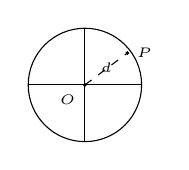
\begin{tikzpicture}[scale=0.45]
\draw (0,0) circle (1.6);
\draw (-1.6,0) -- (1.6,0);
\draw (0,-1.6) -- (0,1.6);
\draw[dashed] (0,0) -- (1.2,0.9);
\node at (0.6,0.5) {\tiny $d$};
\draw[fill=black] (0,0) circle (1pt) node[below left]{\tiny $O$};
\draw (1.2,0.9) circle (1pt) node[right]{\tiny $P$};
\end{tikzpicture}
\end{minipage}



\ans{C) $5\sqrt2$}
\method{$O_1=(-2,3)$, $O_2=(7,-6)$, $O_1O_2=\sqrt{9^2+9^2}=9\sqrt2$, $r_1=3\sqrt2$, $r_2=\sqrt2$, sum $4\sqrt2$, shortest $=9\sqrt2-4\sqrt2=5\sqrt2$. Externally separated ($d>r_1+r_2$).}
\inv{Shortest = centre distance minus sum of radii (external). If one circle contained the other, it would be $|r_1-r_2|-d$. For these numbers, $5\sqrt2\approx7.07$.}

%── D2 ──────────────────────────────────────────────────────────────────────────
\item The segment joining $(3,3)$ and $(7,5)$ is a diameter of circle $C$. $C$ is translated $3$ left, reflected in the $x$-axis, then enlarged scale factor $4$ about its centre. What is the equation of the final circle? \textit{\small(after TMUA Specimen Paper 1 Q9)}
\begin{itemize}
\item[A)] $(x-2)^2+(y-4)^2=80$
\item[B)] $(x-2)^2+(y+4)^2=80$
\item[C)] $(x-2)^2+(y-4)^2=320$
\item[D)] $(x-2)^2+(y+4)^2=320$
\end{itemize}

\ans{B) $(x-2)^2+(y+4)^2=80$}
\method{Original centre $(5,4)$, $r^2=(2)^2+1^2=5$. Translate $3$ left: $(2,4)$, reflect in $x$-axis: $(2,-4)$, enlarge $4\times$ about centre: $r^2=5\cdot16=80$, so $(x-2)^2+(y+4)^2=80$.}
\inv{Enlargement about the centre leaves the centre fixed and multiplies the radius by $4$, so $r^2$ by $16$. The $320$ options scale $r^2$ by $64$ (radius by $8$). Where would the centre go if the enlargement were about the origin instead?}

%── D3 ───────────────────────────────────────────────────────────────────────
\item A circle has centre $O$ and radius $6$. Points $P$ and $Q$ lie on it with $\angle POQ\ge 90^\circ$, and triangle $POQ$ has area $9\sqrt3$. The point $R$ moves on the major arc $PQ$. What is the greatest possible area of triangle $PRQ$? \textit{\small(adapted from TMUA 2022 Paper 1 Q14)}
\begin{itemize}
\item[A)] $18+9\sqrt3$
\item[B)] $27\sqrt3$
\item[C)] $27+9\sqrt3$
\item[D)] $36+9\sqrt3$
\end{itemize}

\ans{B) $27\sqrt3$}
\method{$[POQ]=\tfrac12\cdot36\sin\theta=9\sqrt3$ gives $\sin\theta=\tfrac{\sqrt3}{2}$, and $\theta\ge90^\circ$ forces $\theta=120^\circ$. Then $PQ=6\sqrt3$ and $O$ is $3$ from $PQ$. $R$ is farthest from $PQ$ at the far end of the diameter through the midpoint, at height $6+3=9$, so the area is $\tfrac12\cdot6\sqrt3\cdot9=27\sqrt3$. Option A is the answer if you take $\theta=60^\circ$.}
\inv{The condition $\angle POQ\ge90^\circ$ is doing real work: $\sin60^\circ=\sin120^\circ$. Check that $\theta=60^\circ$ gives the same $[POQ]$ but a greatest area of $18+9\sqrt3$.}

%── D4 ───────────────────────────────────────────────────────────────────────
\item Two tangents are drawn from the origin to the circle $(x-5)^2+(y-5)^2=5$. What is the tangent of the acute angle between them?
\begin{itemize}
\item[A)] $\tfrac34$
\item[B)] $\tfrac43$
\item[C)] $\tfrac52$
\item[D)] $1$
\end{itemize}

\ans{A) $\tfrac34$}
\method{The origin is $\sqrt{50}$ from the centre and $r=\sqrt5$, so half the angle has $\sin\tfrac\theta2=\tfrac{1}{\sqrt{10}}$ and $\tan\tfrac\theta2=\tfrac13$. Then $\tan\theta=\dfrac{2/3}{1-1/9}=\tfrac34$. Check: the tangents $y=mx$ need $\tfrac{|5m-5|}{\sqrt{m^2+1}}=\sqrt5$, so $2m^2-5m+2=0$ and $m=2$ or $\tfrac12$, and $\tfrac{2-1/2}{1+1}=\tfrac34$. Option C is the sum of the gradients, option D their product, option B the reciprocal.}
\inv{The two gradients multiply to $1$. What does that say about how the two tangents sit relative to the line $y=x$, and why does the symmetry of the circle force it?}

%── D5 ───────────────────────────────────────────────────────────────────────
\item The circle through $(0,0)$, $(8,0)$ and $(2,6)$ meets the $y$-axis again at $Q$. How far is $Q$ from the origin?
\begin{itemize}
\item[A)] $2\sqrt5$
\item[B)] $6$
\item[C)] $2$
\item[D)] $4$
\end{itemize}

\ans{D) $4$}
\method{The centre is on $x=4$ (perpendicular bisector of the first two points). Equidistance from $(0,0)$ and $(2,6)$: $16+b^2=4+(6-b)^2$ gives $b=2$, so the centre is $(4,2)$ and $r^2=20$. On $x=0$: $(y-2)^2=4$, so $y=0$ or $4$, and $Q=(0,4)$. Option A is the radius; option C is the centre's height.}
\inv{Get $OQ$ without the centre: the power of the origin is zero, so use the equation $x^2+y^2+2gx+2fy=0$ and substitute the other two points. Which coefficient gives $OQ$ directly?}

\end{enumerate}

%═══════════════════════════════════════════════════════════════════════════════
\section*{Top 5 Patterns --- Worksheet \#2}
\begin{enumerate}[leftmargin=2em, itemsep=4pt]
  \item \textbf{Complete the square before anything else.} Centre $(-g,-f)$, $r^2=g^2+f^2-c$; never trust a radius you have not computed. \seealso{A1, A2, B2, C4, C5}
  \item \textbf{Tangency is a distance statement.} A line is tangent exactly when the centre is $r$ from it; never substitute the line into the circle. \seealso{B6, B8, C8, D4}
  \item \textbf{Tangent $\perp$ radius.} At a point of the circle, the tangent's gradient is the negative reciprocal of the radius's; on $x^2+y^2=r^2$ it is $xx_1+yy_1=r^2$. \seealso{A7, B3, C1}
  \item \textbf{Half-chord $=\sqrt{r^2-d^2}$.} The perpendicular from the centre bisects every chord. \seealso{A10, B7, B10, C7}
  \item \textbf{Go through the centre.} Nearest and farthest points of a circle, and the gap between two circles, all lie on lines through centres. \seealso{C3, D1, D3}
\end{enumerate}

\section*{Common Traps --- Worksheet \#2}
\begin{enumerate}[leftmargin=2em, itemsep=4pt]
  \item \textbf{Guessing the radius.} Nice-looking centres do not mean a nice radius: $x^2+y^2-18x-22y+178=0$ has $r^2=24$. \seealso{C4}
  \item \textbf{Stopping at the centre.} The distance to the centre is not the distance to the circle; subtract (or add) $r$. \seealso{C3, D1}
  \item \textbf{Confusing the gradients with the angle.} The sum or product of the two tangent gradients is not the angle between them. \seealso{D4}
  \item \textbf{$\sin\theta$ has two angles.} $\sin60^\circ=\sin120^\circ$; read every condition in the question before choosing. \seealso{D3}
  \item \textbf{Dropping the constant.} The constant term decides the radius, whether the circle is real, and whether it passes through the origin. \seealso{A2, B2, B4, C5}
\end{enumerate}

\SpeedClosing{``Tangency is a distance statement in disguise: compare $d$ to $r$, never solve the intersection.''}

\end{document}
